% For Dutch text, use option `dutch'
% For VU students, use option `vu'
\documentclass[12pt,vu]{adammath}
%\documentclass[12pt,vu,dutch]{adammath}

\DeclareOldFontCommand{\bf}{\normalfont\bfseries}{\mathbf}

\usepackage[utf8]{inputenc}

%\usepackage[dutch]{babel}
\usepackage{graphicx}
\usepackage{lipsum}

\usepackage{amsmath}
\usepackage{amssymb}
\usepackage{amsthm}

\usepackage{pgfplots}
\pgfplotsset{compat=newest}
\pgfmathdeclarefunction{gauss}{2}{\pgfmathparse{1/(#2*sqrt(2*pi))*exp(-((x-#1)^2)/(2*#2^2))}}

\usepackage{mdframed}
\newmdenv[
  %% topline=false,
  %% bottomline=false,
  %% rightline=false,
  %% skipabove=\topsep,
  %% skipbelow=\topsep
]{mybox}

\usepackage{listings}

\newcommand\ddfrac[2]{\frac{\displaystyle #1}{\displaystyle #2}}
\newcommand\kl[2]{{\text{KL}({#1} \mid\mid {#2})}}
\newcommand\D[3]{{\text{D}_{#1}({#2} \mid\mid {#3})}}
\newcommand\Da[2]{\D{\alpha}{#1}{#2}}
\DeclareMathOperator*{\argmin}{arg\,min}
\DeclareMathOperator*{\argmax}{arg\,max}
%\usepackage[pdfborder={0 0 0}]{hyperref}
\usepackage{hyperref}

%
% Data
%

\title{Diverging Posteriors \\
\large The practical-minded road to approximate inference}
\author[ven500@student.vu.nl, 2509763]{Victor van den Elzen}
%\author[ingrid.de.vries@vu.nl, 8123102]{Ingrid de Vries}
%\what{Bachelorscriptie
\what{Bachelor thesis}

\programme{Bachelor Wiskunde}
%\track{Dynamiische Systemen}

\supervisor{dr.\ Bartek Knapik}
%\secondgrader{dr.\ Bob Planqu\'e}
\coverimage{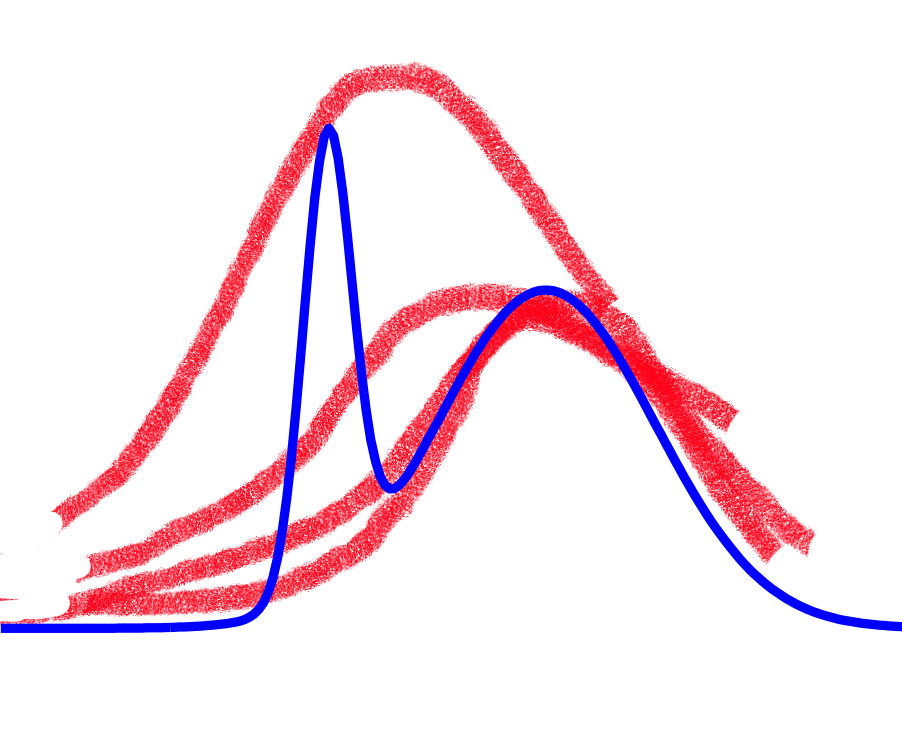
\includegraphics[height=8cm]{cover.png}}

%
% Math environments
%

\theoremstyle{plain}
\newtheorem{theorem}{Theorem}[chapter]
\newtheorem{lemma}[theorem]{Lemma}
\newtheorem*{maintheorem}{Proposition A}  % special theorem

\theoremstyle{definition}
\newtheorem{definition}[theorem]{Definition}
\newtheorem{example}[theorem]{Example}

\theoremstyle{remark}
\newtheorem*{remark}{Remark}

%
% Maths
%

% examples
\newcommand{\field}[1]{\mathbb{#1}}
\newcommand{\R}{\field{R}} % real numbers
\newcommand{\N}{\field{N}} % natural numbers
\newcommand{\C}{\field{C}} % complex numbers
\newcommand{\Z}{\field{Z}} % integers

%
% Content
%

\begin{document}
\maketitle

\begin{abstract}
First, we introduce Bayesian inference and the problem of computation.
We consider symbolic methods, which are limited but fast, and sampling based methods, which are flexible but slow.
Unsatisfied, we introduce the idea of approximate inference, which is behind Variational Bayesian inference and Expectation Propagation.
As background we review Shannon entropy, Kullback-Leibler divergence and $\alpha$-divergence.
We explore that for approximate inference each divergence has different properties and different algorithms.
For solving practical problems, one can now make an informed choice between various probabilistic programming languages.
\end{abstract}

\tableofcontents

\chapter{Overview}
A central problem in statistics is the problem of statistical inference:
determining a distribution based on data and some model assumptions.
We will focus only on Bayesian inference, which is the subject of Chapter \ref{bayesinf}.
Bayesian inference is combining a prior distribution with the likelihood of the data using Bayes' theorem to create a posterior distribution.
Given a model, data and prior distributions for the variables in the model we can in principle calculate the posterior distribution over those variables.

In Chapter \ref{bayescomp} we look at the practical problems of calculating the normalizing constant, calculating certain characteristics and marginalizing nuisance variables that we are not interested in.
All of these problems come down to integrating over the posterior distribution.
This is difficult symbolically except in special cases.
It is also difficult numerically except with very few variables because of the curse of dimensionality.
We can sample using a Markov Chain Monte Carlo (MCMC) method, but in practice these methods are quite slow.
It can even give the idea that Bayesian inference is impractical.

A different way to handle these problems is to approximate the distributions involved with easier distributions.
From now we will focus on this way, which is much faster.
The goal is to find the best approximation distribution from some tractable family, like the normal distributions.
But what do we mean by best approximation?
And how do we find it?

To answer these questions, in Chapter \ref{divergences} we review Shannon entropy, Kullback-Leibler divergence and $\alpha$-divergence.
These divergences give us a way to talk about what distributions are good approximations.

In Chapter \ref{optimizing} we see that these divergences are useful in different cases.
The exclusive Kullback-Leibler divergence prefers to approximate one mode.
The inclusive Kullback-Leibler divergence prefers to approximate the mean and variance.
The $\alpha$-divergence is an extension that can choose in between the above two.

The method to optimize the exclusive Kullback-Leibler divergence is called Variational Bayesian inference, which we consider in Section \ref{vbi}.
The method to optimize the inclusive Kullback-Leibler divergence is called Expectation Propagation, which we consider in Section \ref{ep}.
The method to optimize the exclusive Kullback-Leibler divergence is called Power EP, which we consider in Section \ref{powerep}.

With all this knowledge in hand, one can make an informed choice of probabilistic programming language for their inference problem.
We list some for each method in Chapter \ref{ppl}.

\chapter{Bayesian inference}\label{bayesinf}
\section{Inference using Bayes' Theorem}
The goal of statistical inference is to make statements about probabilities and distributions based on limited data points.

First, recall the following basic theorem of probability (originally \cite{bayes}, modern versions \cite{firstcourse} \S 3.3):
\begin{theorem}[Bayes' Theorem]
Let $A$ and $B$ be events with $P(B) \ne 0$, then
$$P(A|B) = \ddfrac{P(B|A) P(A)}{P(B)}.$$
\end{theorem}
If we know all possible events $A_1, ..., A_n$ of some discrete sample space then
$$P(B) = \sum_{i=1}^n P(B | A_i) P(A_i),$$
which allows us to write
$$P(A_i|B) = \ddfrac{P(B|A_i) P(A_i)}{\sum_{i=1}^n P(B | A_i) P(A_i)}.$$
We are often interested in the probability of some event $E_1$ from a discrete sample space $\{ E_1, ..., E_n \}$ given some data $D$, i.e. $P(E_1 | D)$.
Using Bayes' Theorem we can calculate this if we know two things:
\begin{itemize}
\item the probability of $E_1$ without the data, i.e. $P(E_1)$
\item the probability of $D$ given some event $E_i$, i.e. $P(D | E_i)$
\end{itemize}
That is called Bayesian inference.

\begin{mybox}
\begin{example}\label{discexample}
Say we bought a trick coin that lands on the same ``trick'' side 90\% of the time.
However, we do not know if the trick side is heads or tails, so we try it out and get heads.
What is the probability that the trick side is heads?

Our events are $E_1 = \text{heads is the trick side}$ and $E_2 = \text{tails is the trick side}$.
Our sample space is $\{ E_1, E_2 \}$.
Our data is $D = \text{we got heads}$.

To calculate $P(E_1 | D)$, we first need to know the probability without any data $P(E_1)$.
It seems reasonable to assume that in that case $P(E_1) = P(E_2)$.
Since that's the whole sample space $P(E_1) + P(E_2) = 1$, so $P(E_1) = 0.5$.
We know that $P(D | E_1) = 0.9$ and conversely $P(D | E_2) = 0.1$.
Then
$$P(E_1 | D) = \ddfrac{P(D | E_1) P(E_1)}{P(D | E_1) P(E_1) + P(D | E_2) P(E_2)} = \ddfrac{0.9 \cdot 0.5}{0.9 \cdot 0.5 + 0.1 \cdot 0.5} = 0.9.$$
\end{example}
\end{mybox}

We can write Bayes' Theorem in terms of density functions (\cite{bayesianchoice} \S 1.2).
If we have events $x \in X$ and $y \in Y$, we can replace $P(B|A_i)$ by $f(x | y)$ and $P(A_i)$ by $g(y)$ to get
\begin{theorem}[Bayes' Theorem for discrete distributions]
$$g(y|x) = \ddfrac{f(x | y) g(y)}{\sum_{y \in Y} f(x|y) g(y)}.$$
\end{theorem}

This extends without problems to continuous distributions as
\begin{theorem}[Bayes' Theorem for continuous distributions]\label{eq:bayescont}
$$g(y|x) = \ddfrac{f(x | y) g(y)}{\int_Y f(x|y) g(y) \mathrm{d}y}.$$
\end{theorem}

In Bayesian inference the different terms of Theorem \ref{eq:bayescont} are named.
\begin{itemize}
\item $g(y|x)$ is called the \emph{posterior} distribution.
\item $f(x | y)$ is called the \emph{likelihood} function or the sampling distribution.
\item $g(y)$ is called the \emph{prior} distribution.
\item $\int_Y f(x|y) g(y) \mathrm{d}y$ is called the \emph{normalization factor} or, in some contexts, the partition function.
\end{itemize}

The normalization factor is there so that $g(y|x)$ is a proper distribution with $\int_Y g(y|x) \mathrm{d}y = 1$.
While it can be interesting, we usually leave it implicit as in
$$g(y|x) \propto f(x | y) g(y).$$
Here $\propto$ means that both sides are proportional, that is $g(y|x) = \kappa f(x | y) g(y)$ for some constant $\kappa$.

\begin{mybox}
\begin{example}\label{contexample}
Suppose we have a package and we want to know its weight.
We pick it up and take it to a scale.
Based on the feel we think it is about 5kg, plus or minus 500g.
More formally, our prior is distributed normally like $\mathcal{N}(5, 0.5^2)$ with density function $g(y) \propto e^{-\ddfrac{(y - 5)^2}{2 \cdot 0.5^2}}$.
The scale says it's 4kg, and we know the scale to be accurate to 200g.
Formally, given a certain weight $y$, the results from the scale are distributed like $\mathcal{N}(y, 0.2^2)$.
Then the likelihood of getting 4kg is $f(4 | y) \propto e^{-\ddfrac{(4 - y)^2}{2 \cdot 0.2^2}}$.
So the posterior for the weight being $y$ based on our feel and the scale is
\begin{align*}
  g(y | 4) \propto &f(4 | y) g(y) \propto \\
&e^{-\ddfrac{(4 - y)^2}{2 \cdot 0.2^2}} e^{-\ddfrac{(y - 5)^2}{2 \cdot 0.5^2}} = \\
&e^{-\ddfrac{(4 - y)^2}{2 \cdot 0.2^2} - \ddfrac{(y - 5)^2}{2 \cdot 0.5^2}} = \\
& e^{-\ddfrac{(0.2 + 0.5)y^2 - 2(5 \cdot 0.2^2 + 4 \cdot 0.5^2)y + 5^2 \cdot 0.2^2 + 4^2 \cdot 0.5^2}{2 \cdot 0.2^2 \cdot 0.5^2}} \propto \\
& e^{-\ddfrac{\left(y - \ddfrac{5 \cdot 0.2^2 + 4 \cdot 0.5^2}{0.2^2 + 0.5^2}\right)^2}{2\ddfrac{0.2^2 \cdot 0.5^2}{0.2^2 + 0.5^2}}} = \\
& e^{-\ddfrac{(y - 4.138...)^2}{2 \cdot 0.185...^2}}.
\end{align*}

Our posterior is distributed like $\mathcal{N}(4.138..., 0.185...^2)$.
We can see that our posterior is a combination of the prior and the likelihood (see Figure \ref{fig:contexample}).

We see that the normal distribution has the nice property that when we multiply the density functions of two normal distributions, the result is again the density function of a normal distribution.
In general if $n(\mu, \sigma^2)$ is the density function for $\mathcal{N}(\mu, \sigma^2)$, then
$$n\left(\ddfrac{\mu_1\sigma_2^2 + \mu_2\sigma_1^2}{\sigma_1^2 + \sigma_2^2}, \ddfrac{\sigma_1^2 \sigma_2^2}{\sigma_1^2 + \sigma_2^2}\right) \propto
n\left(\mu_1, \sigma_1^2\right) n\left(\mu_2, \sigma_2^2\right).$$

We can simplify this by using the \emph{precision} instead of the variance with the substitution $\tau = 1 / \sigma^2$ giving
$$n\left((\mu_1 \tau_1 + \mu_2 \tau_2)/(\tau_1 + \tau_2), (\tau_1 + \tau_2)^{-1} \right) \propto
n\left(\mu_1, \tau_1^{-1}\right) n\left(\mu_2, \tau_2^{-1}\right).$$

% http://www.ams.sunysb.edu/~zhu/ams571/Bayesian_Normal.pdf
\end{example}
\end{mybox}

\begin{figure}[h]\label{fig:contexample}
  \centering
  \caption{Illustration of example \ref{contexample}}
\begin{tikzpicture}
  \begin{axis}[smooth,xmin=2,xmax=6,ymin=0,ymax=2.5, cycle list={{blue,solid},{red,dashed},{purple,loosely dashed}}]
    \addplot+[mark=none,domain=2:6,samples=100]{gauss(5, 0.5)};
    \addlegendentry{Prior}
    \addplot+[mark=none,domain=2:6,samples=100]{gauss(4, 0.2)};
    \addlegendentry{Likelihood}
    \addplot+[mark=none,domain=2:6,samples=100]{gauss(4.138, 0.185)};
    \addlegendentry{Posterior}
  \end{axis}
\end{tikzpicture}
\end{figure}

A nice property of Bayes' theorem is that when we have two independent pieces of data such that the likelihood $f(x_1, x_2 | y) = f_1(x_1 | y) f_2(x_2 | y)$ we can do the computation in multiple steps:
$$ g(y | x_1) \propto f_1(x_1 | y) g(y) $$
$$ g(y | x_1, x_2) \propto f_2(x_2 | y) g(y | x_1).$$
Also the the order of these steps does not matter.
This will become crucial in Section \ref{ep} when we consider Expectation propagation.

\section{Reasonable priors}
A key point in getting Bayesian inference off the ground is selecting a reasonable prior distribution.
We can distinguish different kinds of priors:
\begin{itemize}
\item Uninformative or objective priors that try to be unbiased and minimize the information and influence of the prior.
  \begin{itemize}
  \item Priors based on Laplace's Principle of Indifference, like those based on symmetry (such as in Example \ref{discexample}) and maximum entropy (\cite{maxent}, \cite{bayesianchoice} \S 3.2.3).
  \item Priors that minimize information like the Jeffrey's prior which minimizes Fisher information (\cite{jeffreys}, \cite{bayesianchoice} \S 3.5.2).
  \item Priors that maximize the influence of the data like reference priors (\cite{referencepriors}, \cite{bayesianchoice} \S 3.5.4).
  \end{itemize}
\item Informative or subjective priors contain some information not captured by the model.
  This may be considered either problematic or helpful.
  \begin{itemize}
  \item Priors based on ``gut feelings'' or experience that cannot be completely explained (such as in Example \ref{contexample}).
    These may be elicited from subject experts or be personal feelings (\cite{bayesianchoice} \S 3.2.1).
  \item Priors based on data that is related in a way that is not captured by the model.
    For example data from different time periods or similar locations may be used as starting points (\cite{bayesianchoice} \S 3.2.1).
  \item Priors based on the same data as used in the model, known as ``Empirical Bayes''. (\cite{empericalbayes}, \cite{bayesianchoice} \S 10.4).
    This is a bit strange because it is ``double dipping''.
    Empirical Bayes works best when doing many individual inferences on a large amount of data.
  \end{itemize}
\end{itemize}

Some of these priors are not proper distributions and are known as ``improper priors''.

The selection of a prior can be difficult not just mathematically, but also philosophically and when results are to be shared with others.
One piece of good news is the Bernstein-von Mises theorem.
It guarantees that when using parametric models with enough data, the posteriors will converge no matter what (non-pathological) prior is used.
Practically, we can say that if we have a reasonable amount of data the prior is less important and we can get away with any of the above ones.
One strategy is to do an analysis multiple times with different priors.

For the rest of the thesis we will assume a proper prior distribution, and make no more comments on prior selection.

\chapter{Difficulties in practical computation of Bayesian inference}\label{bayescomp}
Looking back on Example \ref{contexample}, multiplying the distribution functions was easy.
We were lucky enough to be able to recognize our posterior as a normal distribution,
which meant we could find our normalization factor $\int_{-\infty}^{\infty} e^{-\frac{(y - 4.138...)^2}{2 \cdot 0.185...^2}} \mathrm{d}y$ easily:
both the trick (looking at the integral multiplied by itself in polar coordinates) and the result ($\sqrt{2\pi\sigma^2}$) are well known.

However, so far this is only for normal priors and normal likelihoods.
Calculating this integral in general is still a problem.

Furthermore, we are often interested not only in the posterior distribution, but also related values.
For example the mean of the posterior distribution is of special interest.
Again, this is an integral over the distribution, this time multiplied by the integrating variable:
$\int_\Omega y g(y | x) \mathrm{d} y$, where $\Omega$ is the sample space of the distribution.
Another thing we might like to look at is the distribution with some variables removed, by integrating them out (marginalization):
$g(y_1 | x) = \int_Y g(y_1, y_2 | x) \mathrm{d} y_2$.

The computation of these kinds of integrals is a central problem in Bayesian inference.

\section{Symbolic computation}
We noticed in Example \ref{contexample} that when our prior and likelihood are both normal distributions, then the posterior is also a normal distribution.

In general if we have a prior from family $\mathcal{P}$ and a likelihood from family $\mathcal{L}$, such that inference gives us a posterior from $\mathcal{P}$, then $\mathcal{P}$ is called a \emph{conjugate prior} to $\mathcal{L}$.
For example the family of normal distributions with a known variance is conjugate prior to itself.
A different example is that the family of beta distributions is conjugate prior to the family of binomial distributions.

When we are in the conjugate prior situation Bayesian inference is quite easy symbolically.
The distributions and integrals are well known, and we can repeat our inference procedure indefinitely.
It is therefore tempting to use these priors when the likelihoods allow it.
However this prior is not always the one we would choose otherwise.
Further, practically we only have useful conjugate priors when the likelihoods are of an exponential family.
That means distributions like binomial, Poisson, normal, Gamma and Beta that we can write as
$$f(x|y) = h(x) e^{\eta(y) \cdot T(x) - A(y)}$$
for some functions $h$, $\eta$, $T$ and $A$.
See \cite{bayesianchoice} \S 3.3 for more information.

When we are not in the conjugate prior situation, symbolically solving the integrals that arise is at least difficult and often impossible.
And even when the symbolic integral is possible, that does not always give us a practical way to compute the numerical value.
See Appendix \ref{code} for a practical implementation of the following examples.

\begin{mybox}
\begin{example}\label{cauchyexample}
Consider the following model: we sample data generated from $\mathcal{C}(\theta, 1)$, a Cauchy distribution with location parameter $\theta$.
That gives us our likelihood.
Our prior on $\theta$ is the standard normal distribution $\mathcal{N}(0, 1^2)$.
Then the posterior given some data $x_1, ..., x_n$ is (\cite{bayesianchoice} Ex 6.1.1)
$$g(\theta | x_1, ..., x_n) \propto e^\frac{-\theta^2}{2} \prod_{i=1}^n \frac{1}{1 + (x_i - \theta)^2}.$$
The normalization constant $Z = \int_{-\infty}^{\infty} g(\theta | x_1, ..., x_n) \mathrm{d} \theta$ cannot be solved symbolically, even allowing special functions like $\texttt{erf}$,
The mean $\int_{-\infty}^{\infty} \theta g(\theta | x_1, ..., x_n) \mathrm{d} \theta / Z$ can also not be solved symbolically.
\end{example}
\end{mybox}

\begin{mybox}
\begin{example}\label{mixtureexample}
Consider the following scenario: to sample, first a biased coin is flipped, then we sample either the left or the right distribution according to the outcome of the coin.
This is a mixture model, a special case of a hierarchical model.
More explicitly call the weight of the biased coin $p$, the left distribution $\mathcal{N}(\mu_1, \sigma_1^2)$ and the right distribution $\mathcal{N}(\mu_2, \sigma_2^2)$.
Let us combine the parameters as $\theta = (p, \mu_1, \sigma_1, \mu_2, \sigma_2)$.
Then the likelihood is $$f(x | \theta) \propto p e^{\frac{-(x-mu_1)^2}{2\sigma_1^2}} + (1-p)e^{\frac{-(x-mu_2)^2}{2\sigma_2^2}}.$$
Finding a prior $g(\theta)$ for all the parameters that makes it possible to symbolically do inference is possible using a combination of the normal, inverse-gamma and beta distributions (\cite{bayesianchoice}, Ex 6.1.5).
Then, skipping over the details, the posterior given data $x_1, ..., x_n$ can be written as
\begin{align*}
  f(\mu_1, \sigma_1, \mu_2, \sigma_2 | x_1, ..., x_n) &\propto g(\theta) \prod_{i=1}^n \left( p e^{\frac{-(x-mu_1)^2}{2\sigma_1^2}} + (1-p)e^{\frac{-(x-mu_2)^2}{2\sigma_2^2}} \right) \\
  &= \sum_{c \in \{\text{left}, \text{right}\}^n} \zeta(c)
\end{align*}
where $\zeta(c)$ is a complicated expression involving special functions for the normal, inverse-gamma and beta distributions.
The most important point is that this posterior involves a sum over every possible choice of left and right for $n$ times, for a total of $2^n$ summation terms.
This means that for larger values of $n$ it becomes practically impossible to actually compute this sum, let alone the normalization constant and the mean!
\end{example}
\end{mybox}

\section{Numerical methods}
When we can't use symbolic integration, we can try to use numerical methods.

For one-dimensional integrals we can simply use the trapezoidal rule or a more advanced technique like Runge-Kutta \cite{rungekutta}.
These involve sampling the function at regularly spaced points.
For example, the total error for Runge-Kutta is proportional to the step size between points $h$, on the order of $h^4$.
On an interval of length $L$ the number of points is $n = L / h$.
This means in practice that numerically computing one-dimensional integrals is very easy and fast.

For higher-dimensional integrals that we get from inference with multiple variables the situation is different.
When we have $d$ dimension and a box like $[0, L]^d$ then a grid of sample points has the number of points $n = (L / h)^d$.
This means that for dimensions higher than about 4 the amount of points needed becomes too high to practically compute (\cite{bayesianchoice}, \S 6.2.1).
Unfortunately different schemes to place points in a regular pattern don't overcome this ``curse of dimensionality''.

Fortunately, our analysis was about the $\textit{total}$ error, but we are usually more interested in the $\textit{relative}$ error.
A grid can still be too much to ask even if we only have 2 points per dimensions, giving a total number of points $n = 2^d$.
One try is to use random points $\theta_1, ..., \theta_n$ sampled from our prior $g(\theta)$ over our space $\Theta$ (for example the box $[0, L]^d$).
Then the normalization factor is $$\int_\Theta f(x | \theta) g(\theta) \mathrm{d}\theta \approx \frac{1}{n} \sum_{i=1}^n f(x | \theta_i).$$
This is called a \emph{Monte Carlo method} due to its randomness, and converges almost surely as $n$ goes to infinity.
If the variance of $g(\theta | x)$ (the posterior) is finite, we can bound the relative error to the order $1/\sqrt{n}$ due to the Central Limit Theorem.

How does this Monte Carlo method do in practice?
A big problem is that often many of the random points are in areas of low probability.
This causes the convergence to be very slow due to high constant factors.
We can try to sample more methodically using stratified sampling methods (\cite{mcmchandbook2} Ch. 8) or give the method a hint with an importance function (\cite{bayesianchoice}, \S 6.2.2).
The most promising method is to pick up hints where to look from the sampled points themselves using $\emph{Markov Chain Monte Carlo}$.

The idea of Markov Chain Monte Carlo (MCMC) is to create a Markov chain which is more likely to go towards areas of high density while still having the average of the points converge to the integral we are looking for (\cite{bayesianchoice} \S 6.3).
Fortunately, such Markov chains turn out to be fairly easy to create in various ways including Metropolis-Hastings methods and Gibbs sampling methods.
They are usually many times faster than Monte Carlo methods and have excellent theoretical convergence properties.
Practically, they are easy to implement and parallelizable.
The success of MCMC for Bayesian inference has made them almost synonymous with Bayesian inference itself.

Still, MCMC is not perfect.
It is not possible to say that any finite sample has converged to or is near the real answer.
There are always unexplored areas of parameter space that may drastically alter the answer.
Further, while MCMC is often fast enough to be practical it is still many times slower than simple symbolic solutions or Frequentist methods that were designed to be calculated by hand.
While it is hard to say anything concrete because every problem is different, we can say that 2 to 10 seconds is on the low end \cite{stanisfast}, up to 30 minutes is possible for more complicated models with hundreds of thousand of data points, and finally there is advice that calculations should be run overnight at least and preferably as long as possible (\cite{mcmchandbook} \S 1.11.3).
These running times are too slow for (soft) real-time use, exploratory data analysis or fitting many different models or data.

\section{Approximate inference - a third way}\label{thirdway}
So far we have seen two methods of computing inference.
The symbolic way can be very fast but is limited in the choice of models and priors.
The MCMC way is somewhat slow but very flexible in the choice of models and priors.
We would like to have something in between those extremes, that we can use when we need something more flexible than symbolic methods but significantly faster than MCMC.

This third way is \emph{approximate inference}, which is the topic for the rest of the thesis.
The idea is to approximate the all distributions by those that can easily be used symbolically, in practice almost always normal distributions.
Then we want to find the best approximation to the posterior distribution.

Approximate inference is fast.
For example, an approximate inference method called ADVI is ``orders of magnitude faster than NUTS, a state-of-the-art MCMC algorithm'' \cite{advi}.
Where MCMC uses minutes, approximate inference uses seconds.
This is a qualitative difference that enables application of Bayesian inference in situations where there is less time or where there are larger problems.

Approximate inference is fairly flexible.
It is applicable when the posterior can be well approximated by a normal distribution.
The likelihoods in many complicated models naturally tend to a normal distribution due to the central limit theorem.
Example \ref{mixtureexample} is an instance of this.
In such a situation, the Bernstein-von Mises theorem tells us that the posterior will also tend to a normal distribution.
Furthermore, we often only want certain characteristics of the posterior like the mean or the variance.
Then ``well approximated'' only means that those characteristics are close.

The big questions then that will be answered in the rest of the thesis are:
\begin{enumerate}
\item What do we mean exactly by ``best approximation''?
\item How do we find the best approximation?
\end{enumerate}

\chapter{Entropy and divergence of distributions}\label{divergences}

\section{Entropy}\label{entropy}
We will first examine the concept of \emph{entropy} as defined by Shannon \cite{shannonentropy}, also know as \emph{Shannon entropy} or \emph{Shannon information}.
In the original formulation, entropy is given by the function $H(p)$ going from a discrete probability distribution $p$ over $\{ 1, ..., n \}$ to a non-negative real number such that
\begin{enumerate}
\item $H$ is continuous in the $p(i)$, and
\item if all $p(i)$ are the same ($1/n$), then $H$ is monotonically increasing in $n$, and
\item the entropy of a joint distribution of two independent distributions is the sum of the entropy of the two independent distributions.
\end{enumerate}
This function is then
\begin{equation}\label{ent}
H(p) = -\sum_{i=1}^n p(i) \log_B p(i)
\end{equation}
which is unique up to a multiplicative constant, namely the base $B$.
$B$ is conventionally set to $2$ or $e$.

The motivation for this definition is in the context of coding information over some communication channel.
With $B = 2$, the expected number of bits needed to communicate a single event from a discrete distribution using the optimal (minimal) code is its entropy.

A different explanation is that $H$ is an increasing function of the number of ways to realize a distribution.
Let's say we have $m$ different objects and buckets of size $m_i = m / p(i)$, where we restrict $m$ such that all $m_i$ are integer.
Dividing the objects between the buckets can be done in $W(m) = \frac{m!}{m_1! ... m_n!}$ different ways.
Then (\cite{ptlos} \S 11.4)
$$\lim_{m \to \infty} \frac{1}{m} \log W(m) = H(p).$$

The extension of the definition of $H$ to a continuous distribution $p(x)$ called \emph{differential entropy} is
\begin{equation}\label{diffent}
H(p) = -\int_{-\infty}^{\infty} p(x) \log_B p(x) \mathrm{d}x.
\end{equation}
There is a subtlety here that Equation \ref{diffent} is not the limit of Equation \ref{ent} for finer and finer discrete distributions $p$, which would be infinite \cite{maxent}.

\begin{mybox}
\begin{example}\label{entropyexample}
The normal distribution is $p(x) = (2\pi\sigma^2)^{-1/2}e^{-\frac{(x - \mu)^2}{2\sigma^2}}$.
Its entropy in base $e$ is
\begin{align*}
H(p) &= -\int_{-\infty}^{\infty} p(x) \log p(x) \mathrm{d}x & \\
&= -\int_{-\infty}^{\infty} p(x) \log \left((2\pi\sigma^2)^{-1/2}e^{-\frac{(x - \mu)^2}{2\sigma^2}}\right) \mathrm{d}x & \\
&= -\int_{-\infty}^{\infty} p(x) \left(-\frac{1}{2} \log (2\pi\sigma^2) + -\frac{(x - \mu)^2}{2\sigma^2}\right) \mathrm{d}x & \\
&= \frac{1}{2} \log (2\pi\sigma^2) \int_{-\infty}^{\infty} p(x) \mathrm{d}x + \frac{1}{2\sigma^2} \underbrace{\int_{-\infty}^{\infty} (x - \mu)^2 p(x) \mathrm{d}x}_{\text{variance}} & \\
&= \frac{1}{2} \log (2\pi\sigma^2) + \frac{1}{2\sigma^2} \sigma^2 & \\
&= \frac{1}{2} \log (2\pi\sigma^2 e). &
\end{align*}
\end{example}
\end{mybox}

\section{Kullback-Leibler divergence}\label{kldivergence}
Building on the idea of entropy, Kullback and Leibler defined the ``information in $x$ for discrimination'' between two distributions $p$ and $q$ as $\log \frac{p(x)}{q(x)}$ \cite{kullback}.

Then the ``mean information for discrimination'' over discrete $p$ is
$$\kl{p}{q} = \sum_{i=1}^n p(i) \log_B \frac{p(i)}{q(i)}.$$
This is what we now call the \emph{Kullback-Leibler divergence} from $q$ to $p$.

We can see this as a more general version of entropy.
Using a uniform distribution $u(x) = 1/n$, the entropy $H(p) = \log_B n - \kl{p}{u}$.
Let us interpret this in terms of coding in base 2.
$H(p)$ is the optimal number of bits to encode $p$.
$\log_2 n$ is the optimal number of bits to encode a uniform distribution.
Then $\kl{p}{u}$ is the number of bits wasted when using the uniform code instead of the optimal code for $p$.
In general, $\kl{p}{q}$ is the number of bits wasted when using the optimal code for $q$ to encode $p$.

Just like entropy, a different explanation is that $\kl{p}{q}$ is a monotone function of the number of ways to realize $p$, but now weighted by the distribution $q$.
The weighted number of ways is $W_q(m) = \frac{m!}{m_1! ... m_n!} q(1)^{m_1} ... q(n)^{m_n}$.
Then (\cite{infcrit} \S 3.1.3)
$$\lim_{m \to \infty} \frac{1}{m} \log W_q(m) = -\kl{p}{q}.$$

For continuous $p$ and $q$ the definition of Kullback-Leibler divergence is
$$\kl{p}{q} = \int_{-\infty}^\infty p(x) \log_B \frac{p(x)}{q(x)} \mathrm{d}x.$$

Kullback-Leibler divergence has many nice properties.
One of them is that $\kl{p}{q} \ge 0$ with $\kl{p}{q} = 0$ if and only if $p = q$ almost everywhere, which is the definition of a \emph{divergence}.
However, the Kullback-Leibler divergence is not symmetric, $\kl{p}{q} \ne \kl{q}{p}$, and it does not obey the triangle inequality in either direction.
So it is not a \emph{metric}.

The asymmetry will be considered in depth when applying the Kullback-Leibler divergence to approximating distributions.

\begin{mybox}
\begin{example}[Moment matching]\label{momentmatching}
What is the best normal approximation to a distribution $p(x)$?
One answer (see Section \ref{incexc}) is that it is the normal distribution with parameters $\mu$ and $\sigma^2$ that minimizes $\kl{p}{\phi(x | \mu, \sigma^2)}$, where
$$\phi(x | \mu, \sigma^2) = \frac{1}{\sqrt{2\pi\sigma^2}}e^{-\ddfrac{(x-\mu)^2}{2\sigma^2}}.$$
We can solve this by finding the stationary points, where the derivatives with respect to $\mu$ and $\sigma^2$ are zero.
Let's look at the derivative with respect to $\mu$:

\begin{align*}
\frac{\mathrm{d}}{\mathrm{d} \mu} \kl{p}{\phi(x | \mu, \sigma^2)} &=
\frac{\mathrm{d}}{\mathrm{d} \mu} \int_{-\infty}^\infty p(x) \log \frac{p(x)}{\phi(x | \mu, \sigma^2)} \mathrm{d} x \\
&= \frac{\mathrm{d}}{\mathrm{d} \mu} - \int_{-\infty}^\infty p(x) \log \phi(x | \mu, \sigma^2) \mathrm{d} x \\
&= \frac{\mathrm{d}}{\mathrm{d} \mu} \int_{-\infty}^\infty p(x) \frac{(x - \mu)^2}{2 \sigma^2} \mathrm{d} x \\
&= -\frac{1}{\sigma^2} \int_{-\infty}^\infty p(x) (x - \mu) \mathrm{d} x \\
&= -\frac{1}{\sigma^2} \left( \int_{-\infty}^\infty x p(x) \mathrm{d} x - \mu \right).
\end{align*}

This derivative is equal to zero exactly when $\mu = \int_{-\infty}^\infty x p(x) \mathrm{d} x$.
The second derivative is $1 / \sigma^2 > 0$, so this is indeed a minimum.
That means that the mean of the best normal approximation is the same as the mean of $p$.

In a similar way we can find that the optimal variance $\sigma^2$ for this $\mu$ is exactly the variance of $p$.
That completely determines the normal distribution.

Approximating $p$ with a normal distribution with the same mean and variance is called \emph{moment matching}.
\end{example}
\end{mybox}

\section{Amari $\alpha$-divergence}\label{alphadivergence}
In the field of information geometry, we have a further generalization of entropy and Kullback-Leibler divergence called $\alpha$-divergence \cite{amari}.
The simplest formula for this divergence is \cite{zhu}
$$\Da{p}{q} = \frac{1}{(1-\alpha)\alpha}\left(1 - \int_{-\infty}^{\infty} p(x)^\alpha q(x)^{1-\alpha} \mathrm{d} x\right).$$
This is a divergence because $\Da{p}{q} \ge 0$ with $\Da{p}{q} = 0$ if and only if $p = q$ almost everywhere.
The values for $\alpha = 0$ and $\alpha = 1$ are defined by continuous extension, which turn out to be
\begin{align*}
\D{1}{p}{q} &= \kl{p}{q}, \text{ and } \\
\D{0}{p}{q} &= \kl{q}{p}.
\end{align*}
In this way the $\alpha$-divergence is an extension of the Kullback-Leibler divergence, which interpolates between the two directions for $\alpha \in (0, 1)$.

The other special value is $\alpha = 1/2$, which is the only value for which the $\alpha$-divergence is symmetric.
In general we have a sort of dual symmetry $\D{\alpha}{p}{q} = \D{1-\alpha}{q}{p}$.

\section{Other divergences}
The Kullback-Leibler divergence is very important and the basis for basically all approximate inference methods.
However, there are other divergences that could be used.
One of the drawbacks of the Kullback-Leibler divergence is that it is not symmetric, and thus not a metric.
The original paper \cite{kullback} suggests the symmetrized version
$$\kl{p}{q} + \kl{q}{p}.$$
A different symmetrized version is Jensen-Shannon divergence \cite{jsd}
$$\kl{p}{\frac{p + q}{2}} + \kl{q}{\frac{p + q}{2}}.$$
We encountered the Hellinger distance already in disguise: \cite{hellinger} \cite{zhu}
$$\text{Hel}^2(p, q) = \frac{1}{2} \int_{-\infty}^\infty \left(\sqrt{p(x)} - \sqrt{q(x)}\right)^2 \mathrm{d} x = \frac{1}{4}\D{1/2}{p}{q}.$$
The Wasserstein distance or the Earth Mover Distance is a metric that has recently been used in machine learning problems \cite{wassersteingan}:
$$\inf_{\gamma \in \Pi(p, q)} \text{E}_{(x, y) \sim y} \lVert x - y \rVert.$$

One might also look to different generalizations of the Kullback-Leibler divergence such as the confusingly similar Rényi $\alpha$-divergence \cite{renyi}:
$$\frac{1}{1-\alpha} \int_{-\infty}^{\infty} p(x)^{\alpha} q(x)^{1-\alpha} \mathrm{d}x.$$
This divergence is also equal to to $\kl{p}{q}$ when $\alpha = 1$, but unlike the Amari $\alpha$-divergence it has no connection to the Kullback-Leibler divergence for $\alpha = 0$.

\chapter{Approximations using different divergences}\label{optimizing}
Now that we know some divergences we can try to answer the first question raised in section \ref{thirdway}:
what do we mean exactly by ``best approximation''?

The standard answer is that we mean the approximation with the minimal Kullback-Leibler divergence to the true posterior.
However, there is an ambiguity here.
Let's say we have a posterior $g(y | x)$ and an approximation $\tilde{g}(y | x)$ from some tractable family like the normal distribution.
Should we minimize $\kl{g}{\tilde{g}}$ or $\kl{\tilde{g}}{g}$?
Following \cite{minkadiv} we will call $\kl{g}{\tilde{g}}$ the \emph{inclusive} and $\kl{\tilde{g}}{g}$ the \emph{exclusive} divergence, for reasons made clear below.

From an interpretational point of view, $\kl{g}{\tilde{g}}$ seems to make the most sense.
We often consider the first argument of the Kullback-Leibler divergence to be the ``true'' distribution, and the second argument the mistaken or simplified model (e.g. \cite{infcrit}).

From a practical point of view, we will examine the inclusive and exclusive divergence on an example and see that they are appropriate for different characteristics.
Then we will examine the optimization problems generated by the inclusive and exclusive divergence.

\section{Inclusive and exclusive divergence}\label{incexc}
The difference between the inclusive and exclusive divergence is most clear in an example that can't be well-approximated by a normal distribution.
In Figure \ref{f:minka}, we see what happens with the best approximation of a mixture of two normal distributions by a single normal distribution.

\begin{figure}\label{f:minka}
  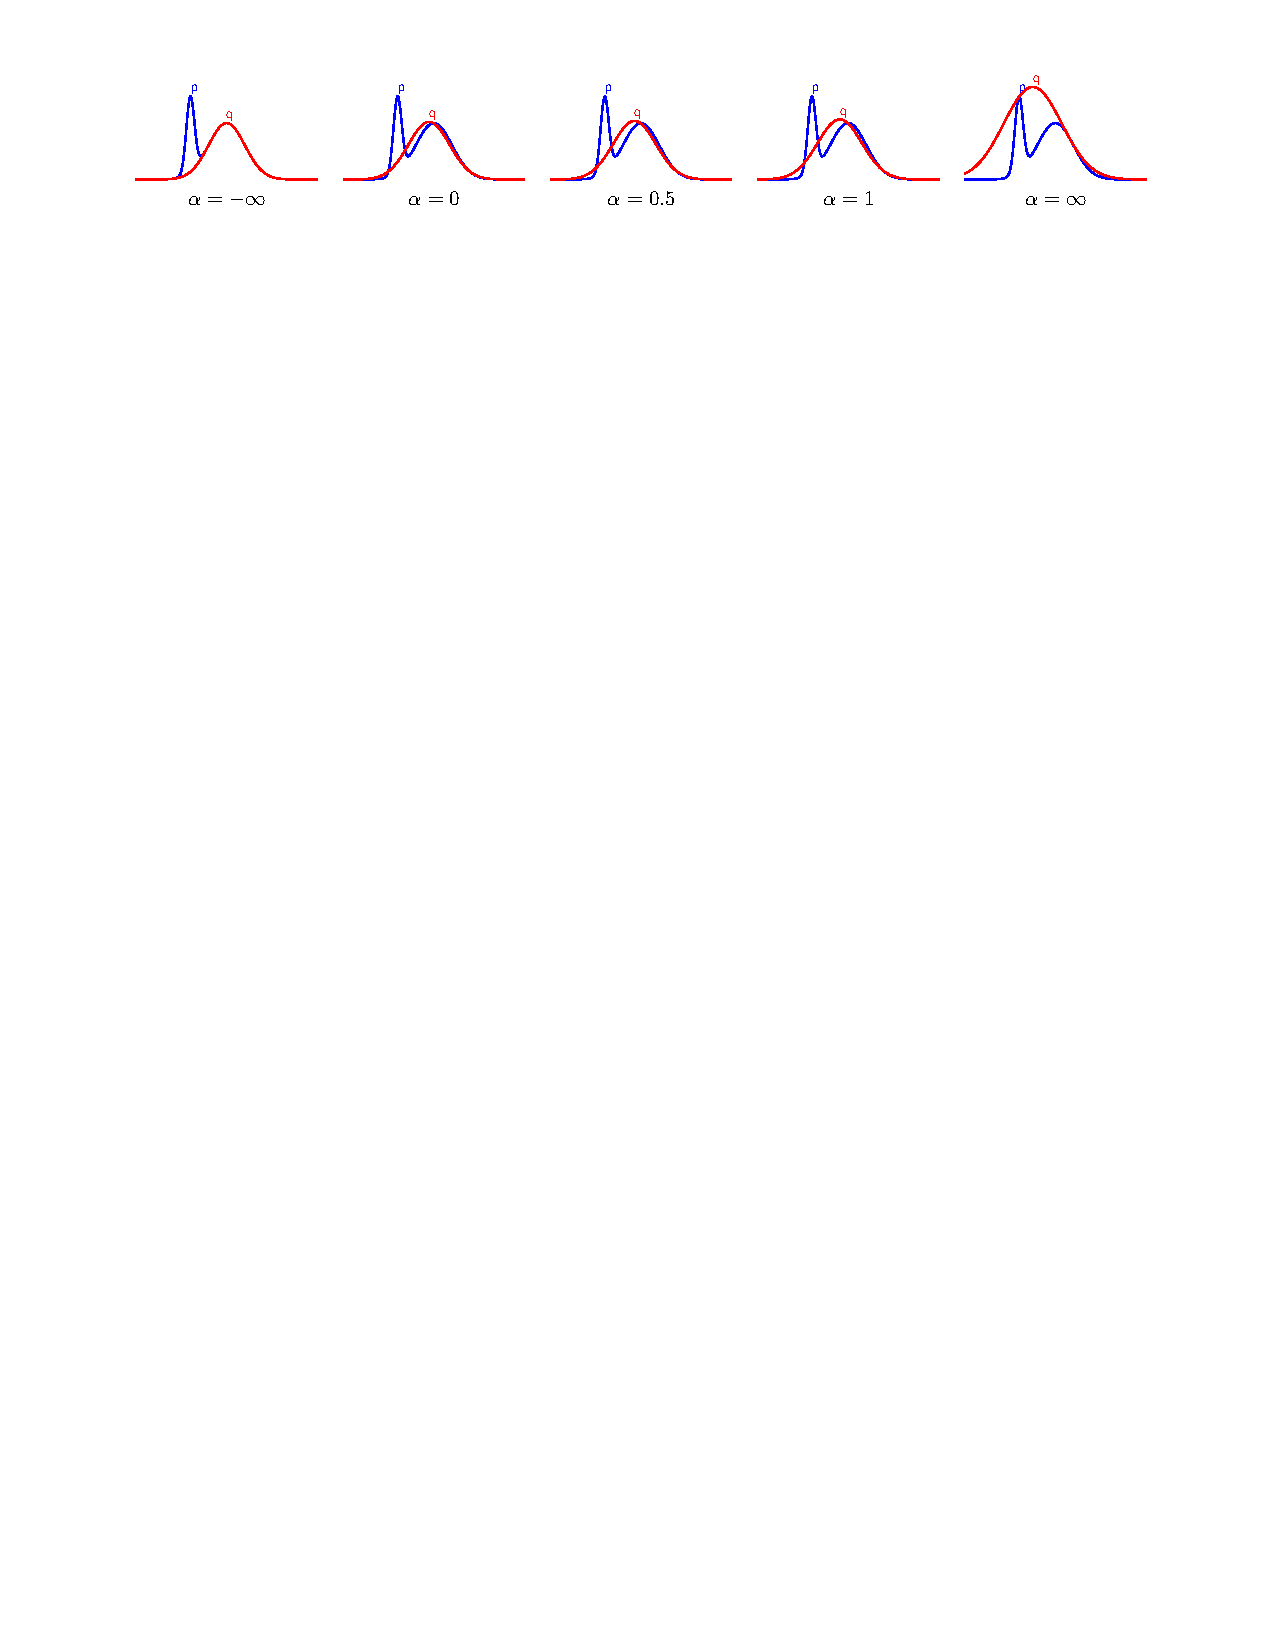
\includegraphics[width=\textwidth]{figures/from-minka-divergence.pdf}
  \caption{The best normal approximation for a mixture for different values of $\alpha$.
    $\alpha = 0$ corresponds to the exclusive divergence.
    $\alpha = 1$ corresponds to the inclusive divergence.
    Image copied from \cite{minkadiv}.}
\end{figure}

We can see that the inclusive divergence tries to capture both parts of the mixture while the exclusive divergence only captures one part.
This is exaggerated at more extreme values of $\alpha$.
We can explain this by looking at the form of the divergences.

For the inclusive divergence
$$\kl{g}{\tilde{g}} = \int_{-\infty}^\infty g(y|x) \log \frac{g(y|x)}{\tilde{g}(y|x)} \mathrm{d}x,$$
the divergence goes to infinity when $\tilde{g}$ is zero but $g$ is not zero in some region.
So the best approximation will have mass anywhere the true posterior has mass.
We call this behavior \emph{zero avoiding}.

On the other hand for the exclusive divergence
$$\kl{\tilde{g}}{g} = \int_{-\infty}^\infty \tilde{g}(y|x) \log \frac{\tilde{g}(y|x)}{g(y|x)} \mathrm{d}x$$
the divergence goes to infinity when $g$ is zero but $\tilde{g}$ is not zero in some region.
So the best approximation will have \emph{no} mass anywhere the true posterior has \emph{no} mass.
We call this behavior \emph{zero forcing}.

These behaviors extend to the $\alpha$-divergence
$$\Da{g}{\tilde{g}} = \frac{1}{(1-\alpha)\alpha}\left(1 - \int_{-\infty}^{\infty} \frac{g(x)^\alpha}{\tilde{g}(x)^{\alpha-1}} \mathrm{d} x\right).$$
When $\alpha > 1$, the $\alpha$-divergence is zero avoiding.
When $\alpha < 0$, the $\alpha$-divergence is zero forcing.

In terms of characteristics, the inclusive divergence is the one that has the correct mean and variance \cite{minkadiv}.
In fact the normal distribution that minimizes the inclusive divergence has the same mean and variance as the true posterior.
That is known as moment matching, see Example \ref{momentmatching}.
However, the maximum (mode) of the inclusive divergence is often very different from the true posterior.
The exclusive divergence gives us a distribution where the maximum is close to a local maximum of the true posterior, namely the maximum of the part of the mixture with the most weight.

These properties give us an idea of when we should use each divergence.
We will come back to this choice when examining the best $\alpha$ for $\alpha$-divergence minimization.

\section{Variational Bayesian inference (exclusive)}\label{vbi}
The approximate inference method that optimizes the exclusive divergence is called variational Bayesian inference, sometimes Variational Inference (VI) or Variational Bayes (VB) for short.
The optimization problem is
$$\argmin_{\tilde{g} \in \mathcal{F}} \kl{\tilde{g}}{g}.$$
Here $\mathcal{F}$ is some tractable family.
Although more complicated families are possible, to be concrete we will use the so called \emph{mean-field approximation} where our approximations are fully factored normal distributions.
Then
$$\tilde{g}(y|x) = \tilde{g}(\mu_1, ..., \mu_n, \sigma_i, ..., \sigma_n | x_1, ..., x_n) = \prod_{i=1}^n \frac{1}{\sqrt {2\pi \sigma_i^2}} e^{-{\ddfrac {(x_i-\mu_i )^{2}}{2\sigma_i^2}}}$$
for some $\mu_i, \sigma_i$ which are the variables that we will optimize.

Now the first problem is that we do not know what $g(y|x)$ is exactly.
Indeed the whole point is to avoid having to calculate the normalization factor $Z_g = \int_Y f(x|y) g(y) \mathrm{d}y$!
However we know the denormalized part $f(x | y) g(y) = g(y|x) Z_g$.
So let us rewrite our optimization objective in terms of the what we know:
\begin{align*}
  \kl{\tilde{g}}{g} & = \int_Y \tilde{g}(y | x) \log \frac{\tilde{g}(y|x)}{g(y|x)} \mathrm{d}y \\
  &= \int_Y \tilde{g}(y | x) \log \tilde{g}(y|x) \mathrm{d}y - \int_Y \tilde{g}(y | x) \log g(y|x) \mathrm{d}y \\
  &= \int_Y \tilde{g}(y | x) \log \tilde{g}(y|x) \mathrm{d}y - \int_Y \tilde{g}(y | x) \log \frac{g(y|x) Z_g}{Z_g} \mathrm{d}y \\
  &= \int_Y \tilde{g}(y | x) \log \tilde{g}(y|x) \mathrm{d}y - \int_Y \tilde{g}(y | x) \log (g(y|x) Z_g) \mathrm{d}y + \int_Y \tilde{g}(y | x) \log Z_g \mathrm{d}y \\
  &= \int_Y \tilde{g}(y | x) \log \tilde{g}(y|x) \mathrm{d}y - \int_Y \tilde{g}(y | x) \log (g(y|x) Z_g) \mathrm{d}y + \log Z_g.
\end{align*}
Because the Kullback-Leibler divergence is non-negative
$$\text{ELBO}(\tilde{g}) = \int_Y \tilde{g}(y | x) \log (g(y|x) Z_g) \mathrm{d}y - \int_Y \tilde{g}(y | x) \log \tilde{g}(y|x) \mathrm{d}y$$
is a lower bound for $\log Z_p$, where ELBO stands for ``evidence lower bound'' \cite{varinf2016}.
Also because $\log Z_g$ is constant with respect to $\tilde{g}$, for optimization we can use the ELBO like
$$\argmin_{\tilde{g} \in \mathcal{F}} \kl{\tilde{g}}{g} = \argmax_{\tilde{g} \in \mathcal{F}} \text{ELBO}(\tilde{g}).$$

Now the last term of the ELBO is just the entropy of $\tilde{g}$ which is usually well known.
In our specific case it is the sum of the entropy of normal distributions, $\sum_{i=1}^n \log \sqrt{2 \pi e \sigma_i^2}$.

So the last problem is the term $\int_Y \tilde{g}(y | x) \log (g(y|x) Z_g) \mathrm{d}y$.
Sometimes $g(y|x) Z_g = f(x|y) g(y)$ has a form that is simplified by the logarithm, like a product of exponential family distributions:
$$\log \prod_{i=1}^n h_i(x) e^{\eta_i(y) \cdot T_i(x) - A_i(y)} = \sum_{i=1}^n \left( \log h_i(x) + \eta_i(y) \cdot T_i(x) - A_i(y) \right).$$
In that case, we can often symbolically find an optimization scheme \cite{vmp}.
For example, our mean-field approximation lets us derive a coordinate descent scheme \cite{varinf2016}.
But even when $g(y|x) Z_g$ is complicated, we can use a Monte Carlo method to find a noisy but unbiased estimate of the gradient of the ELBO with respect to the $y$ \cite{advi} \cite{bbvi}.
Then using these estimated gradients we can optimize $\tilde{g}$ using stochastic gradient descent \cite{bottou}.

One final remark is that unfortunately this optimization problem is generally not convex \cite{varinf2016}.
It is not the fault of the Kullback-Leibler divergence which is convex in both its arguments, but of our space $\mathcal{F}$.
A linear combination of normal distributions is not a normal distribution again, but rather a mixture of normal distributions.
This means that the optimization methods above are not guaranteed to find the global optimum.
Indeed, often they will find a local optimum instead.
The exact optimum found depends on the starting point and the details of the optimization process.
Luckily these local optima are usually close to the global optimum, so the method is still practical.

\section{Expectation Propagation (inclusive)}\label{ep}
The approximate inference method that optimizes the inclusive divergence is called Expectation Propagation (EP).
The optimization problem is
$$\argmin_{\tilde{g} \in \mathcal{F}} \kl{g}{\tilde{g}}.$$
Like in \ref{vbi} we will take $\mathcal{F}$ to be the tractable family of fully factored normal distributions.

The trick used in \ref{vbi} doesn't quite work the same way.
Let's write out our optimization objective in terms of $g(y|x) Z_g$:
\begin{align*}
  \kl{g}{\tilde{g}} & = \int_Y g(y | x) \log \frac{g(y|x)}{\tilde{g}(y|x)} \mathrm{d}y \\
  &= \int_Y g(y | x) \log g(y|x) \mathrm{d}y - \int_Y g(y | x) \log \tilde{g}(y|x) \mathrm{d}y \\
  &= \int_Y g(y | x) \log g(y|x) \mathrm{d}y - \frac{1}{Z_g} \int_Y g(y | x) Z_g \log \tilde{g}(y|x) \mathrm{d}y
\end{align*}

The first term is the entropy of the true posterior, which we can ignore for optimization purposes because it is constant with respect to $\tilde{g}$.
That leaves an unknown multiplicative constant, and $\int_Y g(y | x) Z_g \log \tilde{g}(y|x) \mathrm{d}y$, a different integral than in \ref{vbi}.
In this case the logarithm does not simplify $g(y | x) Z_g$, so this integral is just as hard if not harder than the integral for $Z_g$.
A numerical method based on unbiased estimators of the gradients of $g(y | x)$ with respect to the $y$ has not been developed in the literature.

Instead of trying to optimize the inclusive divergence directly, Expectation Propagation optimizes the \emph{dual} optimization problem \cite{minkaenergy} \cite{wain} based on the dual form of the Kullback-Leibler divergence
\begin{align*}
  \kl{g}{\tilde{g}} = \int_Y g(y|x) \frac{g(y|x)}{\tilde{g}(y|x)} \mathrm{d}y = \max_v \int_Y g(y|x) v(y) \mathrm{d}y - \log \int_Y \tilde{g}(y|x) e^{v(y)} \mathrm{d}y.
\end{align*}
It was not immediately recognized that this was the case, because it's quite technical.
Instead, Expectation Propagation was developed based on a simpler heuristic idea.

One of the first thing that comes to mind when considering approximate inference is to simply approximate the prior $g(y)$ and the likelihood $f(x|y)$ with normal distributions, for example using moment matching.
Then $g(y|x) \approx \tilde{g}(y|x) \propto \tilde{f}(x|y) \tilde{g}(y)$.
This works but the approximation is poor.
When we have multiple independent data points this idea turns into
\begin{equation}\label{idea}
  \tilde{g}(y|x) \propto \tilde{g}(y) \prod_{i=1}^n \tilde{f}(x_i|y).
\end{equation}

An improvement is instead to approximate $g(y)$ with $\tilde{g}(y)$, then try to compute the moments of $\tilde{g}(y) f(x_1|y)$ and moment match them with a normal distribution to produce $\tilde{g}(y | x_1)$.
Then we can repeat the procedure with $\tilde{g}(y | x_1)$ and $f(x_2 | y)$ to produce $\tilde{g}(y | x_1, x_2)$, and so forth until $\tilde{g}(y | x_1, ..., x_n)$.
This gives the \emph{Assumed Density Filtering} algorithm \cite{minkathesis}.
Unfortunately this algorithm is sensitive to the order of the data, and the approximation still isn't very good.

The idea of the Expectation Propagation is to start at an initial approximation, like Equation \ref{idea}, and then keep improving \cite{minkathesis}.
Because the prior $g(y)$ has no special computational status compared to the $f(x_i|y)$, we define $t_0(y) = g(y)$ and $t_i(y) = f(x_i|y)$.
Then $g(y|x_1, ... x_n) \propto \prod_{i=0}^n t_i(y)$.
We call $\tilde{t}^{\setminus i} = \prod_{j \ne i} \tilde{t}_j(y)$ the cavity distribution of $t_i$; it can efficiently be computed as $\tilde{g} / \tilde{t}_i$.
To improve an approximation $\tilde{t}_i$ for some $i$, we first compute a new $\tilde{g}$ by moment matching $t_i \tilde{t}^{\setminus i}$ with a normal distribution.
Then we update $\tilde{t}_i$ to be the unique normal distribution such that $\tilde{g} \propto \prod_{i=0}^n \tilde{t}_i(y)$, or equivalently $\tilde{t_i} \propto \tilde{g} / \tilde{t}^{\setminus i}$.
To finish the algorithm, we simply keep improving $\tilde{t}_i$'s until convergence.

The only computational difficulty in the algorithm is matching the moments of $t_i \tilde{t}^{\setminus i}$ with a normal distribution.
We only need the expectation and the variance.
This can be done symbolically for many distributions.
For example, Infer.NET has full support for doing Expectation Propagation using normal, Bernoulli and Poisson distributions among others \cite{infernet}.
A different approach is to compute the expectation and variance numerically \cite{bbalpha}.

Expectation Propagation does not always converge.
When it does not converge, or converges slowly, this is an indication that the posterior is not well approximated.
However, a convergent algorithm may be required, so there exist extensions which always converge \cite{bbalpha}.

\section{$\alpha$-divergence optimization}\label{powerep}
Our final optimization problem is
$$\argmin_{\tilde{g} \in \mathcal{F}} \Da{g}{\tilde{g}}.$$
This generalizes both the exclusive and the inclusive optimization problems.
We might expect to need a new, difficult method to solve this.
But in fact we can solve this optimization problem with a simple modification of Expectation Propagation, called Power EP \cite{minkapowerep}.

Intuitively, we look only at a fraction $\alpha$ of each $\tilde{t}_i$ when improving it.
We define the modified cavity distribution $\tilde{t}_\alpha^{\setminus i} = (\tilde{t}_i)^{1-\alpha} \prod_{j \ne i} \tilde{t}_j$; it can efficiently be computed as $\tilde{g} / (\tilde{t}_i)^\alpha$.
To improve an approximation $\tilde{t}_i$ for some $i$, we first compute a new $\tilde{g}$ by moment matching $(t_i)^\alpha \tilde{t}^{\setminus i}$ with a normal distribution.
Then we update $\tilde{t_i}$ to be the normal distribution proportional to $(\tilde{g} / \tilde{t}_\alpha^{\setminus i})^{1/\alpha}$.

This algorithm works for any $\alpha$ other than $\alpha = 0$, the exclusive divergence.
We can approximate $\alpha = 0$ with very small values of $\alpha$, and in the limit $\alpha \to 0$ this converges \cite{bbalpha}.
This modification can also make the convergence better or the algorithm easier to compute.

A modern version of $\alpha$-divergence optimization is called Black-Box $\alpha$-Divergence Minimization \cite{bbalpha}.
As the name implies, this method works on arbitrary likelihoods and priors by using numerical methods, such as Monte Carlo estimation, automatic differentiation and stochastic gradient descent.
This method is tailored to large data sets, using a simplification called factor tying.
This simplification is accurate in the case of many independent data points, being equal in the limit to infinity.
It serves to make the method convergent and memory-efficient.

In their paper \cite{bbalpha} Hernández-Lobato et al. perform several experiments to see which value of $\alpha$ gives the best result for various problems.
The first experiment is a probit regression where $\alpha = 1$ is very slightly best using the log-likelihood loss (Figure \ref{f:bbalpha}).
The second experiment is a neural network regression where $\alpha = 0.5$ is best using the log-likelihood loss (Figure \ref{f:bbalpha2}).
The third experiment is a neural network classification where $\alpha = -1$ is best using the average test error and the log-likelihood loss (Figure \ref{f:bbalpha3}).
The final experiment is a neural network regression where $\alpha = 0.5$ is best using the average test error and the log-likelihood loss (Figure \ref{f:bbalpha4}).

\begin{figure}[p]\label{f:bbalpha}
  \centering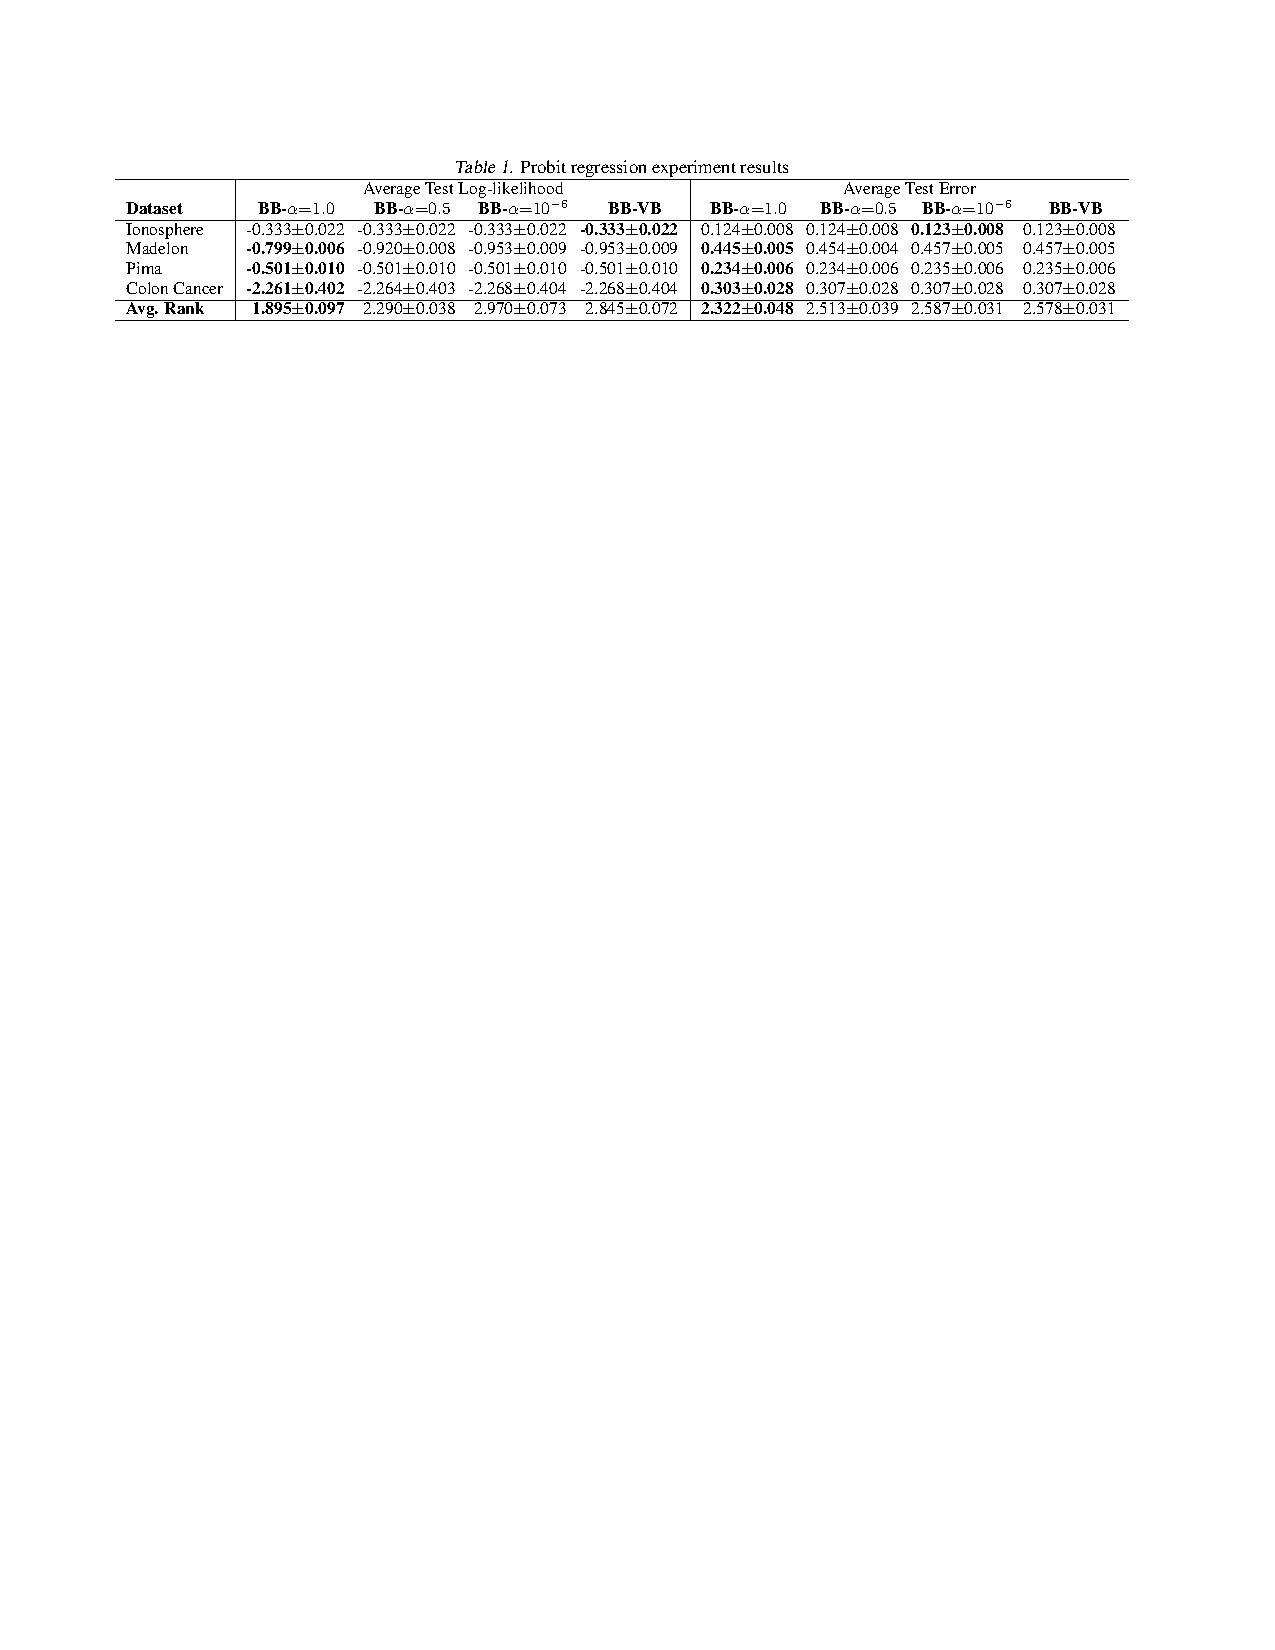
\includegraphics{figures/from-bb-alpha.pdf}
  \caption{First Black-Box $\alpha$-Divergence Minimization experiment results, copied from \cite{bbalpha}.}
\end{figure}
\begin{figure}[p]\label{f:bbalpha2}
  \centering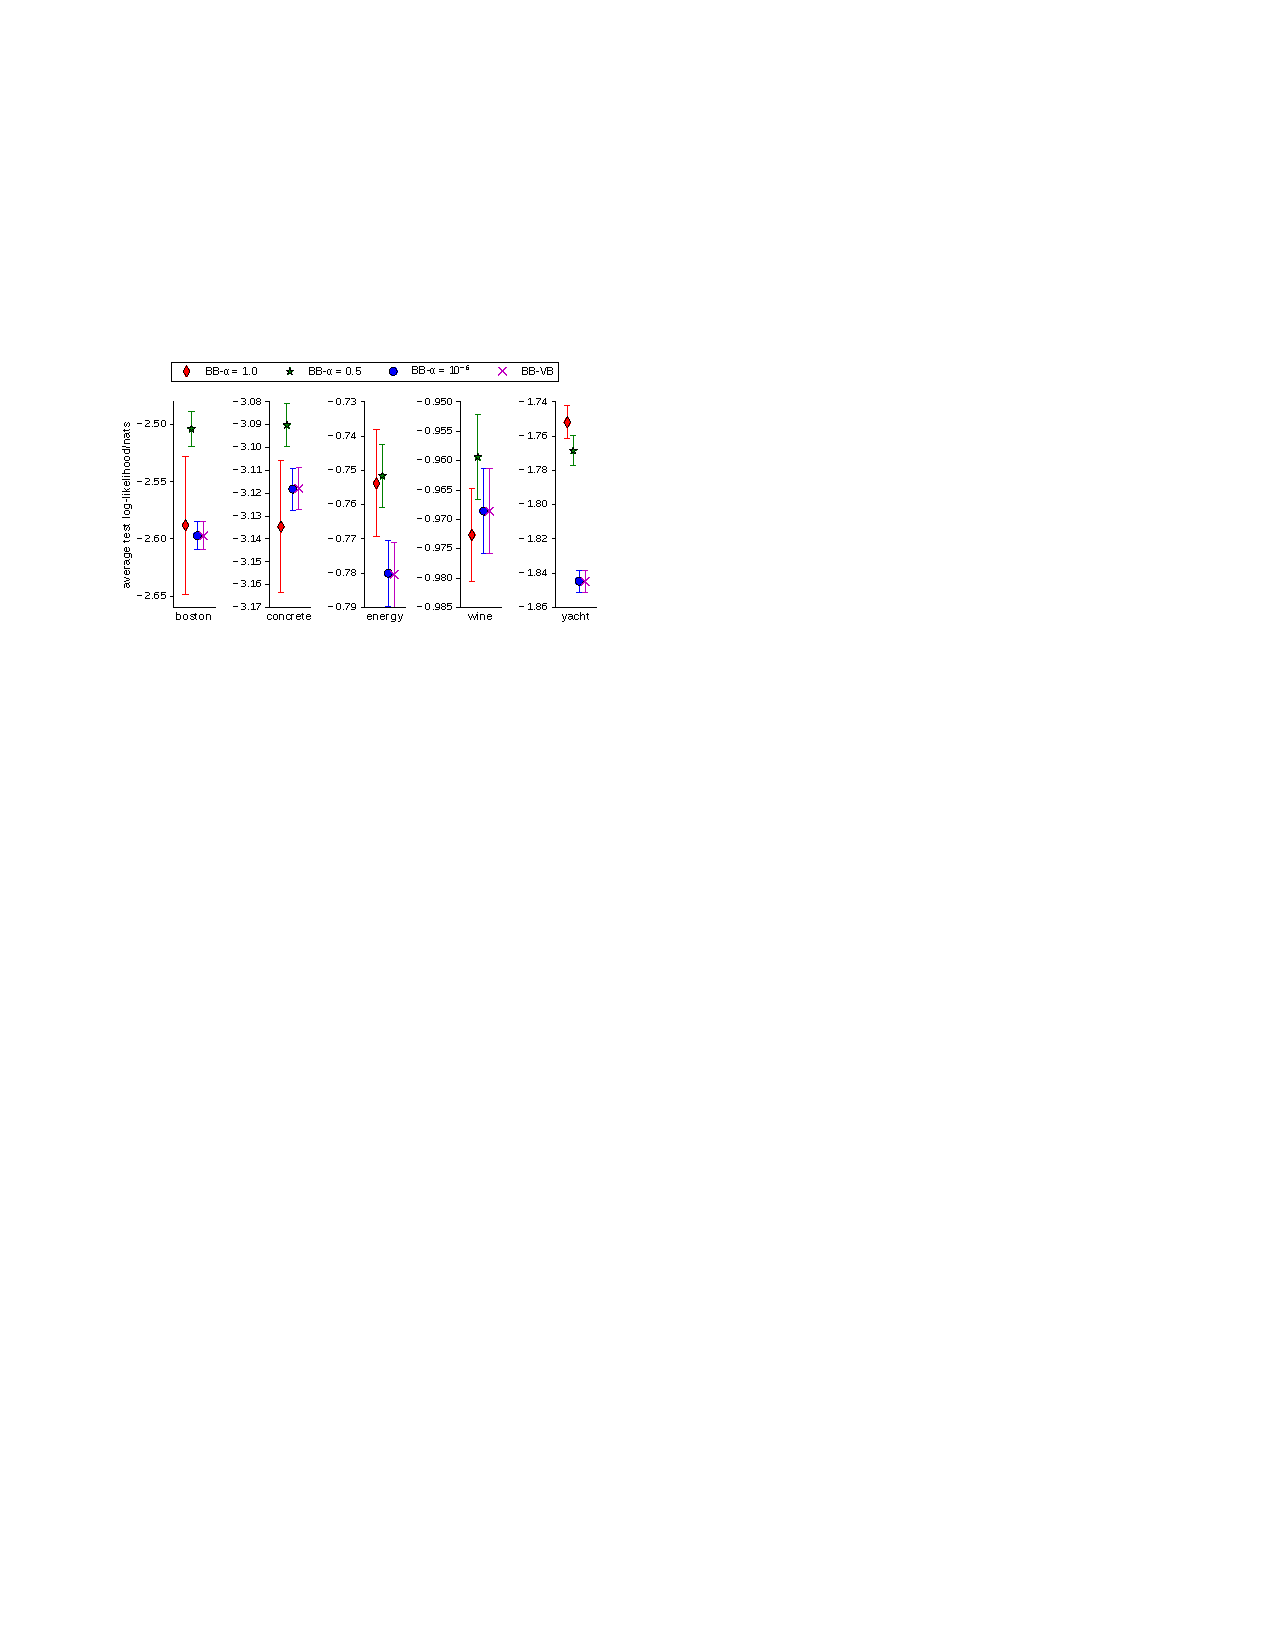
\includegraphics{figures/from-bb-alpha-2.pdf}
  \caption{Second Black-Box $\alpha$-Divergence Minimization experiment results, copied from \cite{bbalpha}.}
\end{figure}
\begin{figure}[p]\label{f:bbalpha3}
  \centering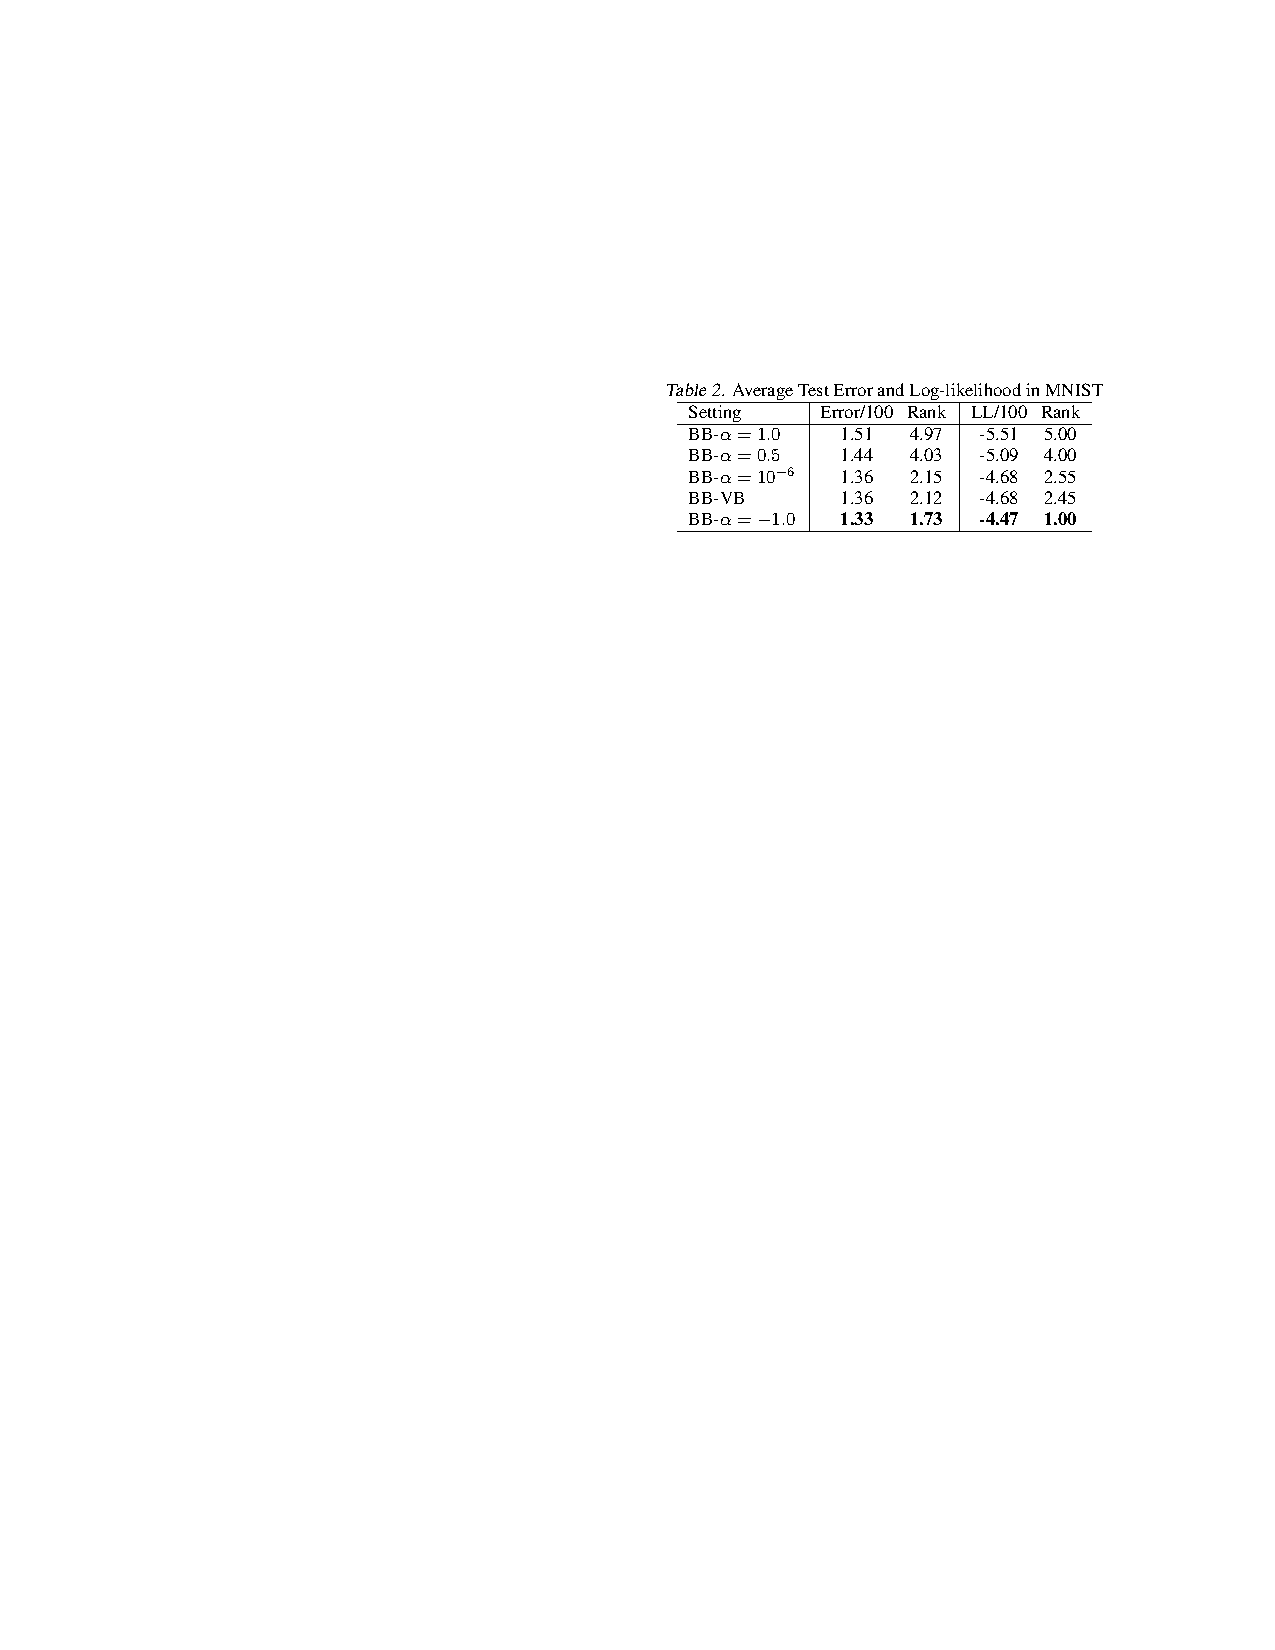
\includegraphics{figures/from-bb-alpha-3.pdf}
  \caption{Third Black-Box $\alpha$-Divergence Minimization experiment results, copied from \cite{bbalpha}.}
\end{figure}
\begin{figure}[p]\label{f:bbalpha4}
  \centering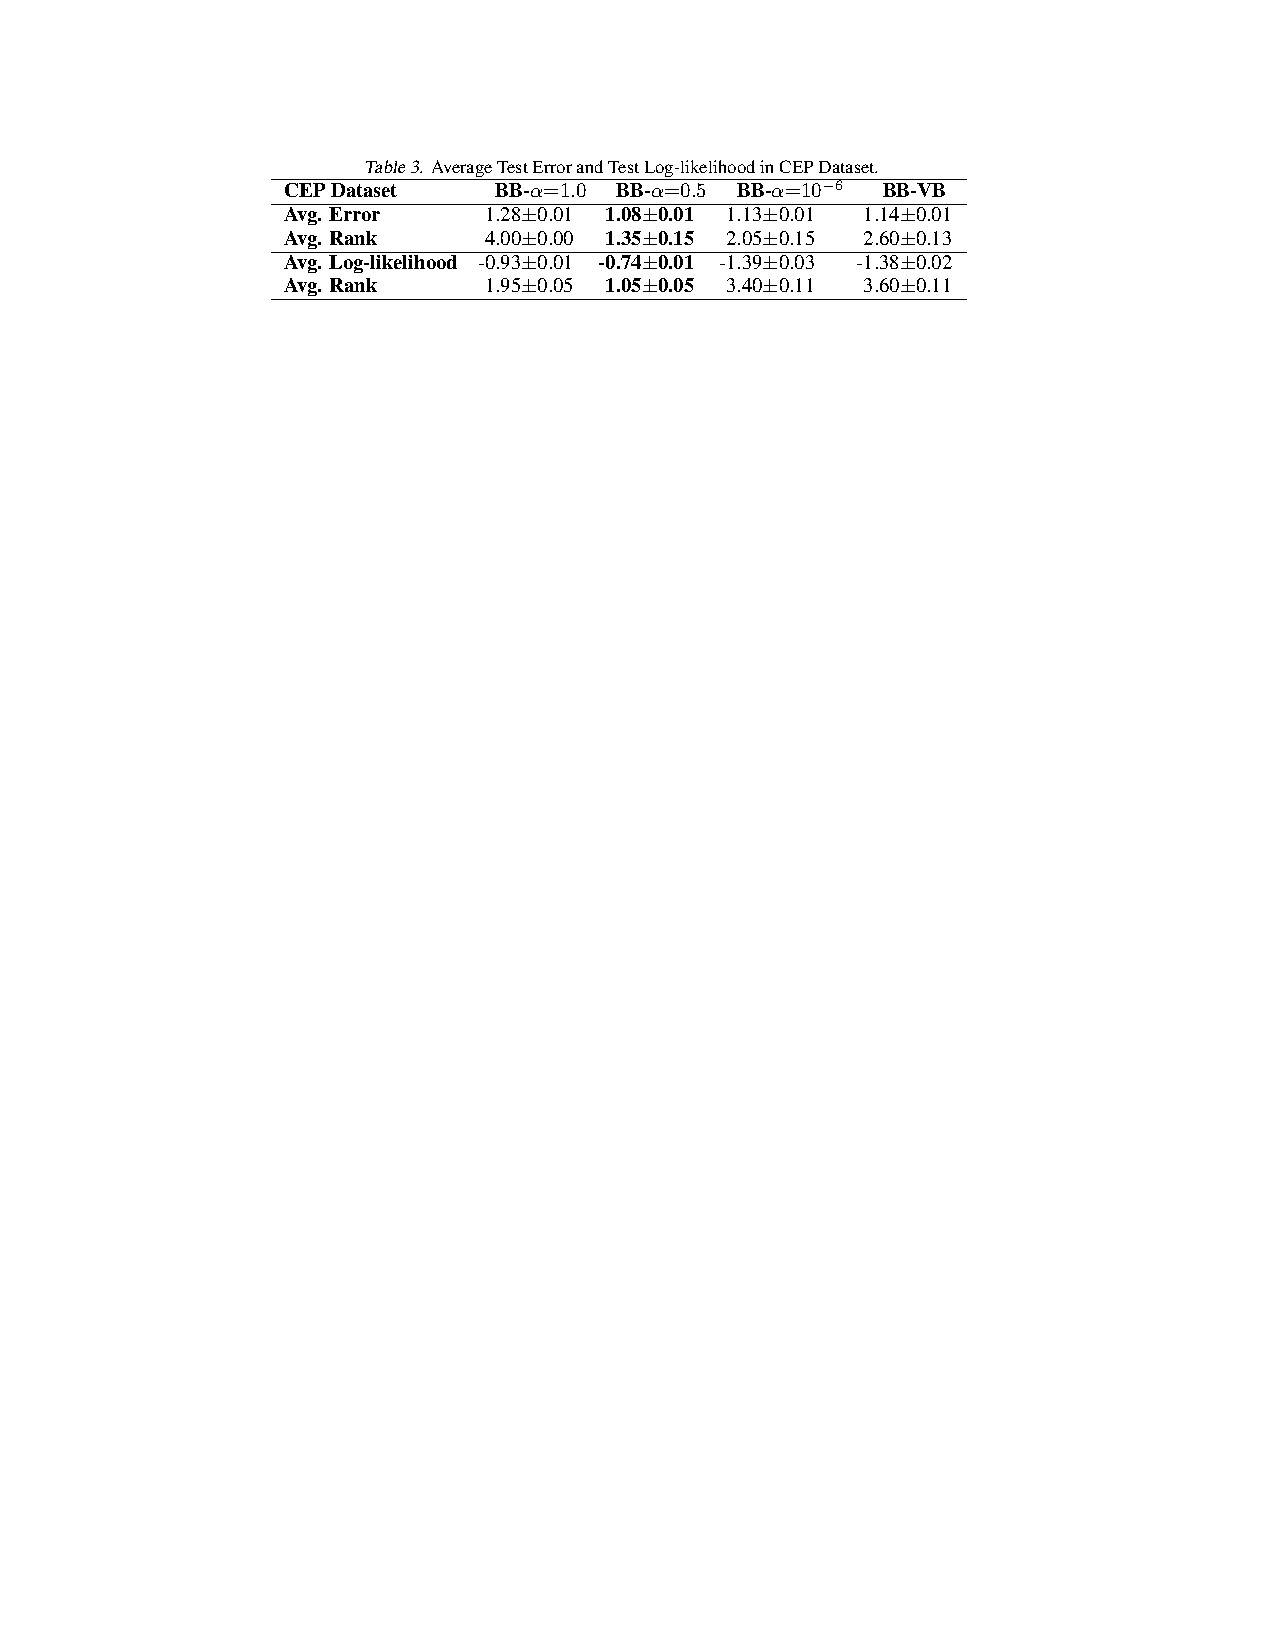
\includegraphics{figures/from-bb-alpha-4.pdf}
  \caption{Fourth Black-Box $\alpha$-Divergence Minimization Black-Box Alpha experiment results, copied from \cite{bbalpha}.}
\end{figure}

As we see there is no single best $\alpha$ value, although $\alpha = 0.5$ (the Hellinger distance) seems like a decent all-round choice.
However, it is clearly valuable to have the ability to choose $\alpha$ according to each problems needs, whether it needs more attention to modes or means.

\chapter{Probabilistic programming languages}\label{ppl}
We considered several methods for Bayesian inference in this thesis.
In passing, a few computer tools were mentioned that can help us apply these methods.
The following tools allow us to describe our model and data in some way and then calculate probabilities and distributions.
They are called \emph{probabilistic programming languages}.

For symbolic methods to inference, we can use general purpose computer algebra systems like Mathematica, Maple and Maxima.
There is also a more specialized tool called PSI Solver (2016, \url{http://psisolver.org}).

For Markov Chain Monte Carlo methods we have several high-quality options:
\begin{itemize}
\item BUGS (1989, \url{http://www.mrc-bsu.cam.ac.uk/software/bugs/})
\item JAGS (2007, \url{http://mcmc-jags.sourceforge.net})
\item Stan (2012, \url{http://mc-stan.org})
\item emcee (2012, \url{http://dan.iel.fm/emcee/})
\end{itemize}

For variational methods (exclusive divergence) we have:
\begin{itemize}
\item ADVI (2015, in Stan \url{http://mc-stan.org})
\item Edward (2016, \url{http://edwardlib.org})
\end{itemize}

For Expectation Propagation (inclusive divergence) we have Infer.NET (2008, \url{http://infernet.azurewebsites.net}).

One can implement any of these algorithms in any programming language.
It may be helpful to use numerical libraries like Eigen and NumPy/SciPy, or machine learning libraries like Tensorflow and Theano.

\chapter{Summary}
We looked at Bayesian inference and its computational problems.

When the model allows for it, we can get exact results using symbolic methods.
For low-dimensional problems we can use standard numerical integration.
For higher-dimensional problems we can use stochastic sampling methods such as Markov Chain Monte Carlo.
When MCMC is too slow, we turn to approximate methods.
We can approximate a mode by optimizing the exclusive divergence using Variational Inference.
We can approximate the mean and variance by optimizing the inclusive divergence using Expectation Propagation.
And we can approximate anything in between by optimizing the $\alpha$-divergence using Power EP.

Finally, we can use a probabilistic programming language to actually perform the computation using the chosen method.

%
% Bibliography
%

% The argument of the thebibliography environment (in this example `x')
% denotes the length of the longest label.
% If you have fewer than 10 references the argument is one character;
% if you have 10 - 99 references you take an argument of two characters.
\begin{thebibliography}{xx}

% Put bibliography in table of contents
\addcontentsline{toc}{chapter}{Bibliography}

\raggedright

\bibitem{amari}
  Shun'ichi Amari,
  \emph{Differential-Geometrical Methods in Statistic},
  1985,
  Springer

\bibitem{wassersteingan}
  Martin Arjovsky, Soumith Chintala, Léon Bottou,
  \emph{Wasserstein GAN},
  2017,
  \url{https://arxiv.org/abs/1701.07875}

\bibitem{bayes}
  Thomas Bayes and Richard Price,
  \emph{An Essay towards solving a Problem in the Doctrine of Chances},
  Philosophical Transactions of the Royal Society of London, \textbf{53}, 370–418,
  1763,
  \url{https://dx.doi.org/10.1098%2Frstl.1763.0053}

\bibitem{referencepriors}
  Jose M. Bernardo,
  \emph{Reference Posterior Distributions for Bayesian Inference},
  1979,
  Journal of the Royal Statistical Society, Series B. \textbf{41}, 113–147,
  \url{http://www.uv.es/~bernardo/1979JRSSB.pdf}

\bibitem{varinf2016}
  David M. Blei, Alp Kucukelbir, Jon D. McAuliffe
  \emph{Variational Inference: A Review for Statisticians},
  2016,
  \url{https://arxiv.org/abs/1601.00670}

\bibitem{bottou}
  L\'eon Bottou,
  \emph{Large-Scale Machine Learning with Stochastic Gradient Descent},
  2010,
  Proceedings of COMPSTAT'2010,
  \url{http://leon.bottou.org/publications/pdf/compstat-2010.pdf}

\bibitem{empericalbayes}
  Bradley Efron,
  2010,
  \emph{Large-Scale Inference: Empirical Bayes Methods for Estimation, Testing and Prediction},
  \url{http://statweb.stanford.edu/~ckirby/brad/LSI/monograph_CUP.pdf}

\bibitem{renyi}
  Tim van Erven,
  \emph{Rényi Divergence and Kullback-Leibler Divergence},
  2014,
  IEEE Transactions on Information Theory, 60 (7)
  \url{https://arxiv.org/abs/1206.2459}

\bibitem{stanisfast}
  Andrew Gelman,
  \emph{Stan is fast},
  2012,
  \url{http://andrewgelman.com/2012/08/30/stan-is-fast/}

\bibitem{mcmchandbook}
  Charles J. Geyer,
  \emph{Introduction to MCMC},
  2011,
  Handbook of Markov Chain Monte Carlo,
  \url{http://www.mcmchandbook.net/HandbookChapter1.pdf}

\bibitem{bbalpha}
  José Miguel Hernández-Lobato, Yingzhen Li, Mark Rowland, Daniel Hernández-Lobato, Thang Bui, Richard E. Turner,
  \emph{Black-box $\alpha$-divergence Minimization},
  2016,
  Proceedings of The 33rd International Conference on Machine Learning, PMLR 48:1511-1520,
  \url{https://arxiv.org/abs/1511.03243}

\bibitem{maxent}
  E. T. Jaynes,
  \emph{Information Theory and Statistical Mechanics},
  1957,
  The Physical Review, \textbf{106} 4, 620-640,
  \url{http://bayes.wustl.edu/etj/articles/theory.1.pdf}

\bibitem{ptlos}
  E. T. Jaynes, G. Larry Bretthorst,
  \emph{Probability Theory: the Logic of Science},
  2003,
  Cambridge

\bibitem{jeffreys}
  H. Jeffreys,
  \emph{An Invariant Form for the Prior Probability in Estimation Problems},
  1946,
  Proceedings of the Royal Society of London. Series A, Mathematical and Physical Sciences. \textbf{186}, 453–461,
  \url{https://dx.doi.org/10.1098%2Frspa.1946.0056}

\bibitem{infcrit}
  Sadanori Konishi, Genshiro Kitagawa,
  \emph{Information Criteria and Statistical Modeling},
  2007,
  Springer

\bibitem{mcmchandbook2}
  Dirk P. Kroese, Thomas Taimre, Zdravko I. Botev,
  \emph{Handbook of Monte Carlo Methods}
  2011,
  Wiley

\bibitem{advi}
  A. Kucukelbir, D. Tran, R. Ranganath, A. Gelman and D.M. Blei,
  \emph{Automatic Differentiation Variational Inference},
  2017,
  Journal of Machine Learning Research, 18(14),
  \url{http://jmlr.org/papers/volume18/16-107/16-107.pdf}

\bibitem{kullback}
  S. Kullback and R.A. Leibler,
  \emph{On information and sufficiency},
  1951,
  Annals of Mathematical Statistics, 22 (1): 79–86,
  \url{https://projecteuclid.org/euclid.aoms/1177729694}

\bibitem{jsd}
  J. Lin,
  \emph{Divergence measures based on the shannon entropy},
  1991.
  IEEE Transactions on Information Theory. 37 (1): 145–151.
  \url{https://www.cise.ufl.edu/~anand/sp06/jensen-shannon.pdf}

\bibitem{minkathesis}
  Thomas Minka,
  \emph{A family of algorithms for approximate Bayesian inference},
  2001,
  Thesis (Ph.D.)--Massachusetts Institute of Technology,
  \url{https://dspace.mit.edu/handle/1721.1/86583}

\bibitem{minkaenergy}
  Thomas Minka,
  \emph{The EP energy function and mimization schemes},
  2001,
  \url{https://tminka.github.io/papers/ep/minka-ep-energy.pdf}

\bibitem{minkapowerep}
  Thomas Minka,
  \emph{Power EP},
  2004,
  Microsoft Research Technical Report MSR-TR-2004-149,
  \url{https://www.microsoft.com/en-us/research/publication/power-ep/}

\bibitem{minkadiv}
  Tom Minka,
  \emph{Divergence Measures and Message Passing},
  2005,
  Microsoft Research Technical Report MSR-TR-2005-173,
  \url{https://www.microsoft.com/en-us/research/publication/divergence-measures-and-message-passing/}


\bibitem{infernet}
  \emph{Infer.NET: List of factors and constraints},
  \url{http://infernet.azurewebsites.net/docs/list\%20of\%20factors\%20and\%20constraints.aspx}

\bibitem{hellinger}
  M.S. Nikulin,
  \emph{Hellinger distance},
  Encyclopedia of Mathematics,
  \url{http://www.encyclopediaofmath.org/index.php?title=Hellinger_distance&oldid=16453}

\bibitem{bbvi}
  Rajesh Ranganath, Sean Gerrish, David M. Blei,
  \emph{Black Box Variational Inference},
  2014,
  \url{http://www.cs.columbia.edu/~blei/papers/RanganathGerrishBlei2014.pdf}

\bibitem{bayesianchoice}
  Christian P. Robert,
  \emph{The Bayesian Choice, 2nd ed.},
  2007,
  Springer

\bibitem{firstcourse}
  Sheldon Ross,
  \emph{A First Course in Probability, 8th ed.},
  2010,
  Pearson

\bibitem{shannonentropy}
  Claude E. Shannon,
  \emph{A Mathematical Theory of Communication},
  1948,
  Bell System Technical Journal, 27 (3),
  \url{http://math.harvard.edu/~ctm/home/text/others/shannon/entropy/entropy.pdf}

\bibitem{wain}
  Martin J. Wainwright and Michael I. Jordan,
  \emph{Graphical Models, Exponential Families, and Variational Inference},
  2008,
  Foundations and Trends® in Machine Learning: Vol. 1: No. 1–2, pp 1-305,
  \url{https://people.eecs.berkeley.edu/~wainwrig/Papers/WaiJor08_FTML.pdf}

\bibitem{rungekutta}
  Eric W. Weisstein,
  \emph{Runge-Kutta Method},
  MathWorld--A Wolfram Web Resource,
  \url{http://mathworld.wolfram.com/Runge-KuttaMethod.html}

\bibitem{vmp}
  John Winn, Christopher M. Bishop,
  \emph{Variational Message Passing},
  2005,
  Journal of Machine Learning Research 6 (661–694),
  \url{http://www.jmlr.org/papers/volume6/winn05a/winn05a.pdf}

\bibitem{zhu}
  Huaiyu Zhu and Richard Rohwer,
  \emph{Information Geometric Measurements of Generalisation},
  1995,
  Technical Report NCRG/4350,
  Aston University,
  \url{http://citeseerx.ist.psu.edu/viewdoc/summary?doi=10.1.1.38.881}
\end{thebibliography}
%
% Appendix
%

\appendix

\chapter{Difficult cases for symbolic inference}\label{code}
We try two difficult symbolic inference problems in PSI Solver commit \verb!da79ca!.
For the Cauchy problem (Example \ref{cauchyexample}) the integral is not solved.
For the mixture problem (Example \ref{mixtureexample}) the time and memory usage grows quickly with the data size, making it practically impossible to compute the solution for more than ten data points.
\lstinputlisting[frame=single,caption=Cauchy problem]{psi/cauchy.psi}
\lstinputlisting[frame=single,caption=Mixture example]{psi/mixture.psi}

\end{document}
